\documentclass[12pt]{article}
\usepackage{amsmath,amssymb,amsthm}
\usepackage{graphicx,mathabx}
\usepackage{xcolor}
\usepackage{tikz}
\usepackage{placeins}
\usepackage{lipsum}
\usepackage[shortlabels]{enumitem}
\begin{document}
\title{TCSS 343 - Challenge 3 - Subset Sum Problem}
\author{Jake McKenzie}
\maketitle
\noindent The key to dynamic programming, at least to me, is to truly write down what steps I need to solve a problem iteratively, ignore the typical recursive step and memoize. Eisenhower put it perfectly: ``No battle was ever won according to plan, but no battle was ever won without one." The first thing to notice is that an optimal dynamic program will have the property no matter the initial state and initial decisions, the corresponding choices the algorithm makes must be the optimal choice for each successive step forward. This is Bellman's principle of optimality.\\\\
\noindent 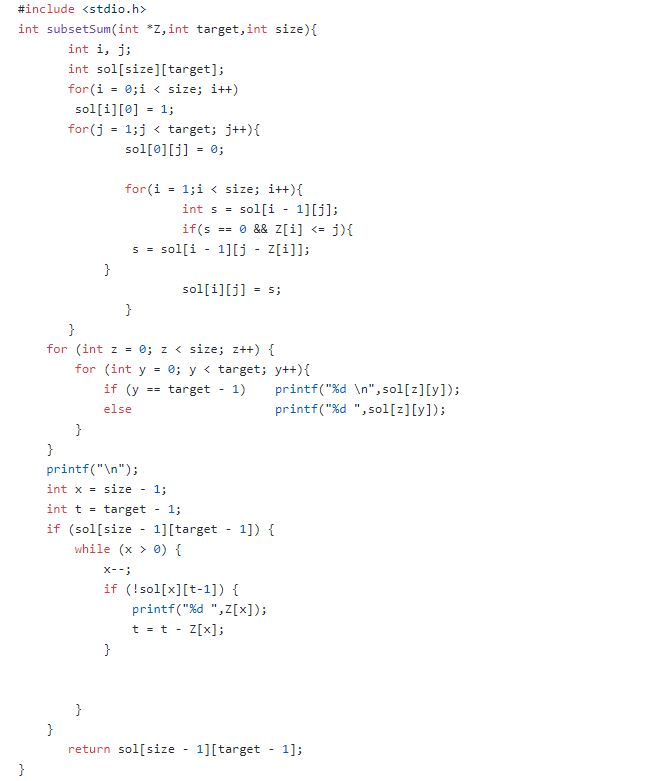
\includegraphics{code1.jpg}\\
\noindent 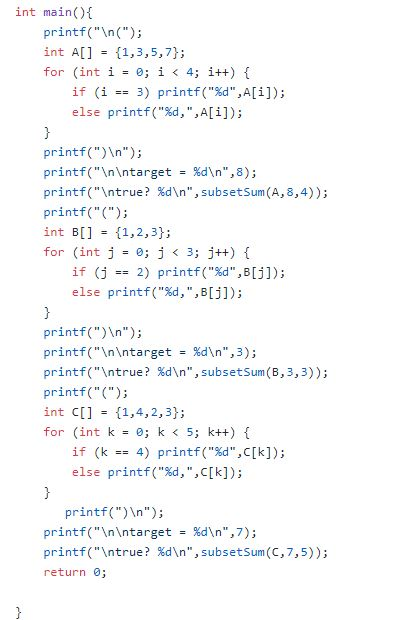
\includegraphics{code2.jpg}\\
\noindent 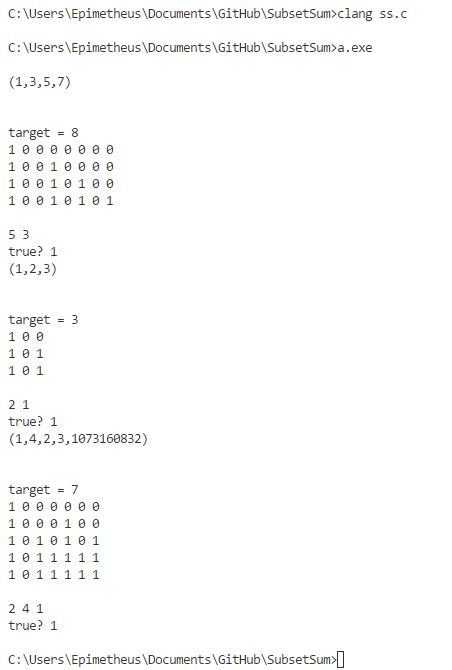
\includegraphics{subsetsum.jpg}\\
\end{document}